\capitulo{3}{Conceptos teóricos}

Esta sección del presente documento tratará dos de los aspectos más importantes en la realización de este trabajo.

La primera parte se centrará en todos los aspectos relacionados con el análisis de datos. Cabe señalar que, para poder emplear en futuros análisis los datos de trayectorias en crudo, obtenidos de distintos usuarios se han de seguir una serie de pasos que permitan limpiarlos y transformarlos en información útil para el sistema. Esta serie de pasos será descrita en esta primera parte de la presente sección.

Por último se verán aspectos relativos al desarrollo de una plataforma web centrada en el usuario donde uno de los aspectos más importantes es la calidad del diseño.



\section{Conceptos previos}
En este apartado se verán los conceptos previos para entender los pasos posteriores aquí detallados.

\subsection{Área}
Toda ruta realizada puede englobarse en un área determinada. Esta área estará marcada por las coordenadas máximas y mínimas de las posiciones que componen la ruta.

Al analizar un conjunto de datos se puede obtener el área formada por todas las posiciones de las rutas que forman el conjunto.

\subsection{Coordenada geográfica}
Una coordenada geográfica está formada por un valor de longitud y un valor de latitud. Estos valores son obtenidos mediante los sistemas GPS o GLONASS (basados en un sistema de satélites y receptores terrestres). El valor de la longitud estará comprendido entre -180.0º y +180.0º, situando la coordenada en el espacio horizontal del globo terrestre. El valor de la latitud sitúa al receptor en el eje vertical y puede tomar valores de entre -90.0º y +90.0º. Siendo el origen de coordenadas el valor formado por la coordenada (0,0).

Además, una coordenada puede contar con otros valores como la marca de tiempo en la que fue tomada o la altura de la misma sobre la superficie terrestre.

\subsection{Ruta}
Cada ruta contará con una serie de coordenadas geográficas que conforman el recorrido que, en este caso, el usuario ha realizado. En la ruta se podrán descubrir \quotes{paradas} (explicado en los siguientes apartados) sobre las que se puedan asignar Puntos De Interés.

El origen y fin de la ruta estará marcado por el orden de las coordenadas geográficas y/o por la marca temporal de las mismas. 

\subsection{Puntos De Interés}
Un PDI o Punto De Interés (en ingles \textit{POI}) permite marcar un lugar representativo o con características relevantes sobre un mapa. Por ejemplo, se pueden marcar lugares de culto, museos, centros comerciales, farmacias, paradas de autobús, hoteles, etc. El número de PDIs sobre un mapa es muy elevado y permite al usuario tomar conciencia de los lugares de interés que le rodean.

Cada PDI podrá contar con distinta información, el nombre propio del lugar, el tipo de lugar, horarios, localización exacta mediante una coordenada geográfica, etc. Es el tipo de lugar el que recibe el nombre de \textit{amenity} y el que será usado como dato relevante en este proyecto.

\subsection{Prueba o ejecución del algoritmo}
Cada una de las ejecuciones del algoritmo será almacenada como una prueba del mismo y permitirá recuperar los datos con los que fue ejecutado. De esta forma se permite visualizar al usuario todas las ejecuciones que ha realizado y los valores de las mismas para así poder variarlos de la forma correcta para que el análisis de los ficheros de datos sea lo más satisfactorio posible.

\section{Análisis de datos de trayectorias geo-espaciales}
Como se ha descrito anteriormente, en este primer apartado de la presente sección se mostrará cómo funciona de forma teórica el algoritmo de análisis de rutas implementado. El primer paso que se ha de dar es el de la limpieza de datos o \textit{data cleaning}. Después se procederá al reconocimiento de las rutas, posteriormente se buscarán paradas y, antes de guardar los resultados, se buscarán Puntos De Interés cercanos a las paradas detectadas. La Figura \ref{esquema} muestra un esquema de funcionamiento del algoritmo.

\begin{figure}[h]
  \centering
    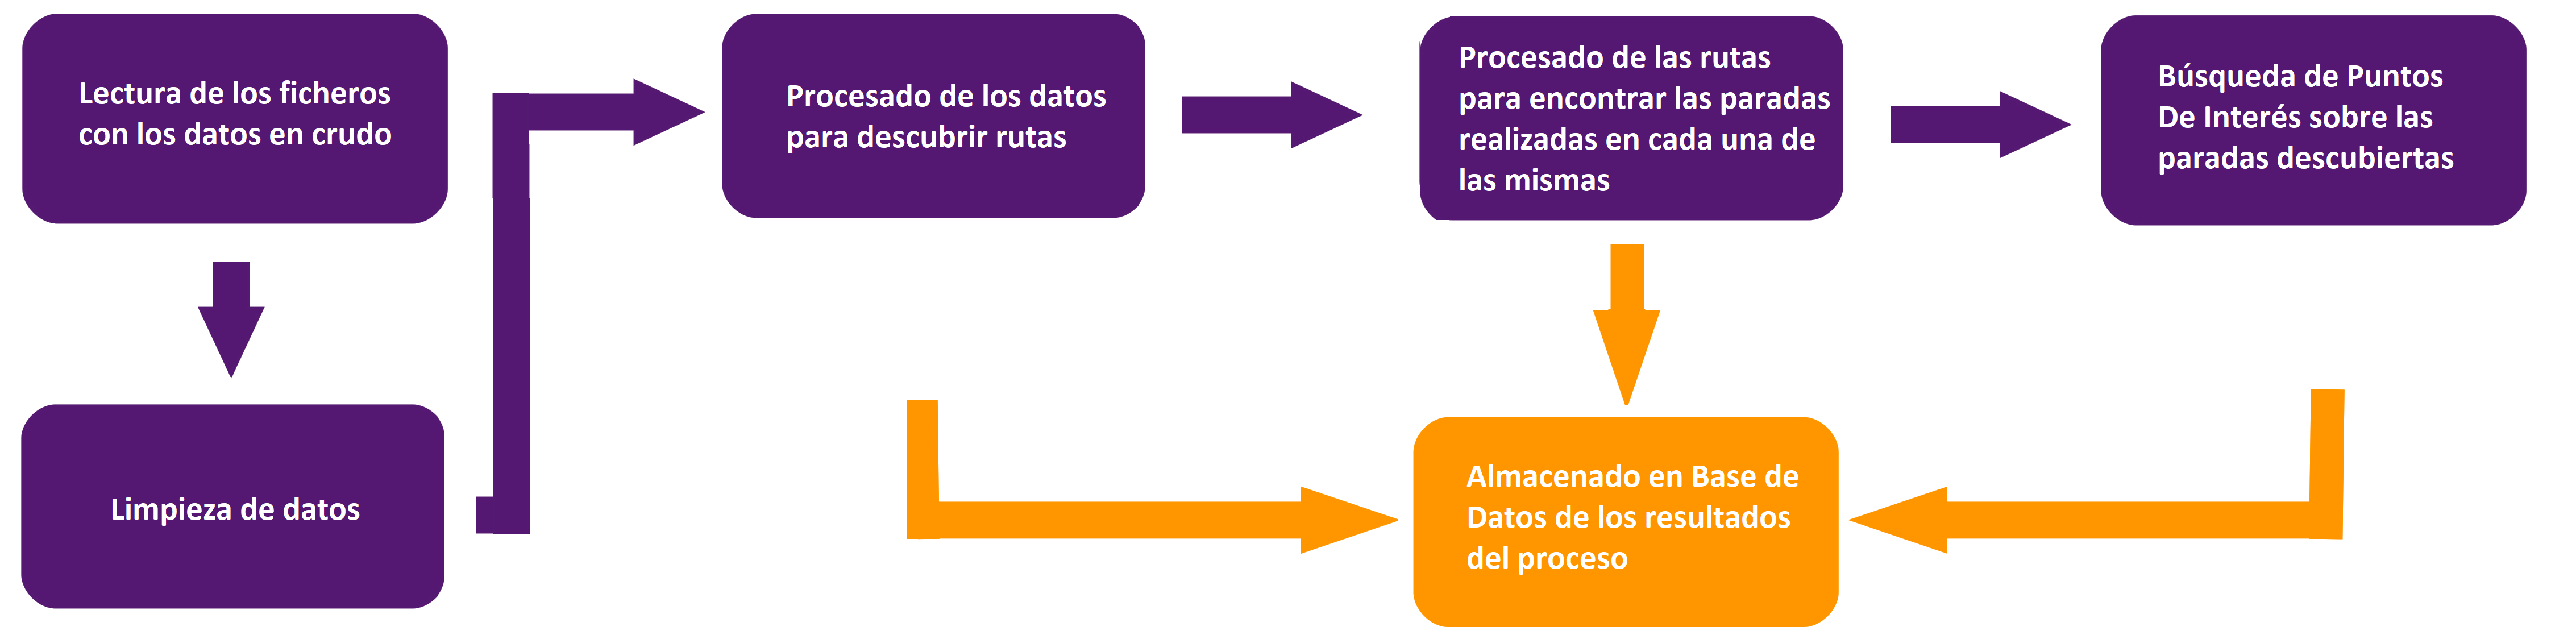
\includegraphics[width=1\textwidth]{../img/diagramas/algoritmo.png}
  \caption{Esquema del algoritmo.}
  \label{esquema}
\end{figure}

A continuación se explica cada uno de los puntos mencionados.

\subsection{Limpieza de datos}

Debido a fallos hardware o software, pueden capturarse rutas que no correspondan con la realidad. Este motivo implica la necesidad de un proceso previo de análisis de los datos para detectar posiciones que no son reales.

Algunos de los problemas que ocasionan que los datos deban pasar por una limpieza previa son los siguientes:

\begin{itemize}
	\item En ocasiones el hardware GPS puede fallar almacenando una posición errónea que no coincide con el resto de posiciones de la ruta.
	\item La precisión de los datos también puede verse afectada por una señal pobre en una zona con mala cobertura GPS.
	\item Este problema también puede ser ocasionado por el software al realizar mal alguno de los cálculos necesarios.
	\item Posiciones inexistentes por no cumplir con las características inherentes a una coordenada GPS. Por ejemplo, su longitud o latitud sobrepasen los límites (-90.0º - +90.0º para la latitud y -180.0º - +180.0º para la longitud).
	\item Falta de posiciones intermedias al haberse perdido la conexión y dándose una unión entre puntos de una ruta poco realista, generando una línea recta entre dos puntos cuando en condiciones normales dicha línea debería ser sustituida por puntos adicionales.
\end{itemize}

\subsubsection{Reconocimiento de rutas en cada fichero y asignación de área}
Una vez eliminadas las posibles posiciones irreales, el siguiente paso es el reconocimiento de las rutas que existen en el fichero analizado. Dentro de un fichero pueden convivir una o varias rutas dependiendo de la actividad del usuario. Estas rutas han de poder ser encontradas y reconocidas.

En este caso, el algoritmo trata de descubrir estas rutas mediante el cálculo de la mediana temporal aportado por cada marca de tiempo de las posiciones. Una vez obtenida dicha mediana, esta será comparada con las diferencias temporales entre todas las posiciones y, en el caso de encontrarse un gran salto temporal, se calculará el salto espacial entre las posiciones tan alejadas temporalmente. Si estas posiciones, además de estar separadas temporalmente, sobrepasan el umbral espacial marcado al algoritmo, las rutas se considerarán distintas y serán separadas.

Este cálculo se realizará con las rutas restantes y se obtendrá el total de rutas existentes en los ficheros analizados.

Una vez reconocida cada una de las rutas y, dependiendo de las opciones seleccionadas por el usuario, se asignará un área a dichas rutas.

Dependiendo de la opción, se seguirá uno de estos dos caminos:

\begin{itemize}
	\item Asignación de una área existente: se asignarán todas las rutas analizadas en la ejecución actual a un área ya existente en la Base de Datos. Esta opción es válida si se conoce cuál es el ámbito de las rutas analizadas y se tiene la certeza de que sus coordenadas cumplen con los límites del área seleccionada.
	\item Creación de una nueva área: el sistema creará un nuevo área con el nombre y descripción asignadas por el usuario. Las coordenadas se calcularán durante el análisis de las rutas.
\end{itemize}

\subsubsection{Segmentación de la trayectoria}

El siguiente paso consiste en dividir la trayectoria seguida en \quotes{movimiento} y \quotes{paradas}. Un periodo de movimiento es el tiempo en el que la persona se encuentra moviéndose entre dos ubicaciones mientras que un periodo de parada es el tiempo en el que, por ejemplo, la persona se encuentra viendo un lugar de interés.

Estas paradas son detectadas una vez calculada la mediana como se ha comentado en los puntos anteriores. En el caso de que existan posiciones cercanas espacialmente pero separadas en el tiempo. Estas posiciones formarán una parada. Entendiendo como parada la entrada en un lugar de interés, la llegada y salida del puesto de trabajo de la persona que porta el dispositivo, etc.

De esta forma se obtienen paradas dentro de la ruta, contemplando el resto de posiciones como movimiento dentro de la misma.

\subsection{Enriquecimiento semántico}

El último proceso realizable es el correspondiente a la asignación de semántica a la ruta. Los datos obtenidos por el usuario solo incluyen posiciones geográficas tomadas en un instante determinado, es decir, solo se tienen datos como la latitud, longitud y el espacio temporal en el que han sido tomados. En esta etapa se incluye información adicional a estos datos.

Este proceso toma las paradas detectadas en la ruta y las contrasta con las posiciones de los Puntos De Interés almacenados en el sistema. Para ello se toma como límite el radio que marca la distancia máxima al que buscar un PDI.

Un PDI obtenido de Open Street Maps puede contener diversa información, dicha información es aportada por la persona que registra dicho dato dentro de los sistemas OSM. Esta información incluye de forma obligatoria la posición espacial del Punto De Interés pero deja al usuario la posibilidad de añadir más información. Generalmente también se cuenta con un nombre en el idioma nativo de la persona que registra el PDI pero en otras ocasiones también existe un nombre genérico en inglés. Adicionalmente, un nodo suele incluir el tipo al que pertenece, este tipo recibe el nombre de \textit{amenity}. Una \textit{amenity} es una generalización de lugar al que representa el PDI. Por ejemplo, pueden existir museos, lugares de culto, gasolineras, centros comerciales, etc. De esta forma se puede conocer el nombre propio del lugar pero también qué tipo de lugar representa.

Una vez se han obtenido los PDIs cercanos a las paradas, todos los datos serán actualizados en la Base de Datos, permitiendo al usuario recuperarlos en el momento  que desee, mostrando los resultados en la página de resultados de la plataforma.
